
\lecture{Prediction Intervals}{prediction-intervals}
\section{Prediction Intervals}

\title{Prediction Intervals}
\subtitle{What will it be?}

%\author{Kelly Black}
%\institute{Clarkson University}
\date{21 April 2014}

\begin{frame}
  \titlepage
\end{frame}

\begin{frame}
  \frametitle{Outline}
  \tableofcontents[hideothersubsections,sectionstyle=show/hide]
\end{frame}


\subsection{Clicker Quiz}


\iftoggle{clicker}{%
  \begin{frame}
    \frametitle{Clicker Quiz}

    \begin{columns}
      \column{.15\textwidth}

      \begin{tabular}{l|l}
        $X$ & $Y$ \\ \hline
        1 &  -4.7 \\
        2 & -15.4  \\
        3 &  -9.6 \\
        4 & -21.5 
      \end{tabular}

      \column{.44\textwidth}

      \begin{eqnarray*}
        \bar{x} & = & 2.5 \\
        \bar{y} & = & -12.8.
      \end{eqnarray*}

      \column{.44\textwidth}

      \only<1>{%
        \begin{eqnarray*}
          s_{xx} & = & ?, \\
          s_{yy} & = & 158.3, \\
          s_{xy} & = & -22.3.
        \end{eqnarray*}
      }
      \only<2>{%
        \begin{eqnarray*}
          s_{xx} & = & 5, \\
          s_{yy} & = & 158.3, \\
          s_{xy} & = & -22.3.
        \end{eqnarray*}
      }


    \end{columns}


    \vfill

    What is the value of $s_{xx}$? \\
    \begin{tabular}{l@{\hspace{3em}}l@{\hspace{3em}}l}
      A: 0 & B: 2.75 & C: 5
    \end{tabular}

    \vfill
    \vfill
    \vfill

  \end{frame}

}

\subsection{Inference On Predicted Value}

\begin{frame}
  \frametitle{Linear Regression}

    \begin{columns}
      \column{.15\textwidth}

      \begin{tabular}{l|l}
        $X$    & $Y$ \\ \hline
        $x_1$  & $y_1$  \\
        $x_2$  & $y_2$  \\
        \vdots & \vdots  \\
        $x_n$  & $y_n$
      \end{tabular}

      \column{.44\textwidth}

      \begin{eqnarray*}
        \bar{x} \\
        \bar{y} \\
        S_{xx} \\
        S_{yy} \\
        S_{xy} 
        \end{eqnarray*}

      \column{.44\textwidth}
      
      \begin{eqnarray*}
        y & = & m x + b + {\color{red}\epsilon} \\
        {\color{blue}\hat{m}} & = & \frac{S_{xy}}{S_{xx}} \\
        {\color{blue}\hat{b}} & = & \bar{y} - \hat{m} \bar{x}
      \end{eqnarray*}

    \end{columns}


      \only<2>{%

        Question: After calculating $\hat{m}$ and $\hat{b}$ we want to
        estimate the value of $y$ for a given value of $x$. What is
        the value of $y$?

        Problem: It depends on three random variables, $\hat{m}$,
        $\hat{b}$, and $\epsilon$.

      }



\end{frame}

\begin{frame}{The Predicted Value}

  \begin{definition}
    The \textit{predicted value} for $y$ at $x$ is
    \begin{eqnarray*}
      \hat{y} & = & \hat{m} x + \hat{b}.
    \end{eqnarray*}
  \end{definition}

    \only<2>{%
      \centerline{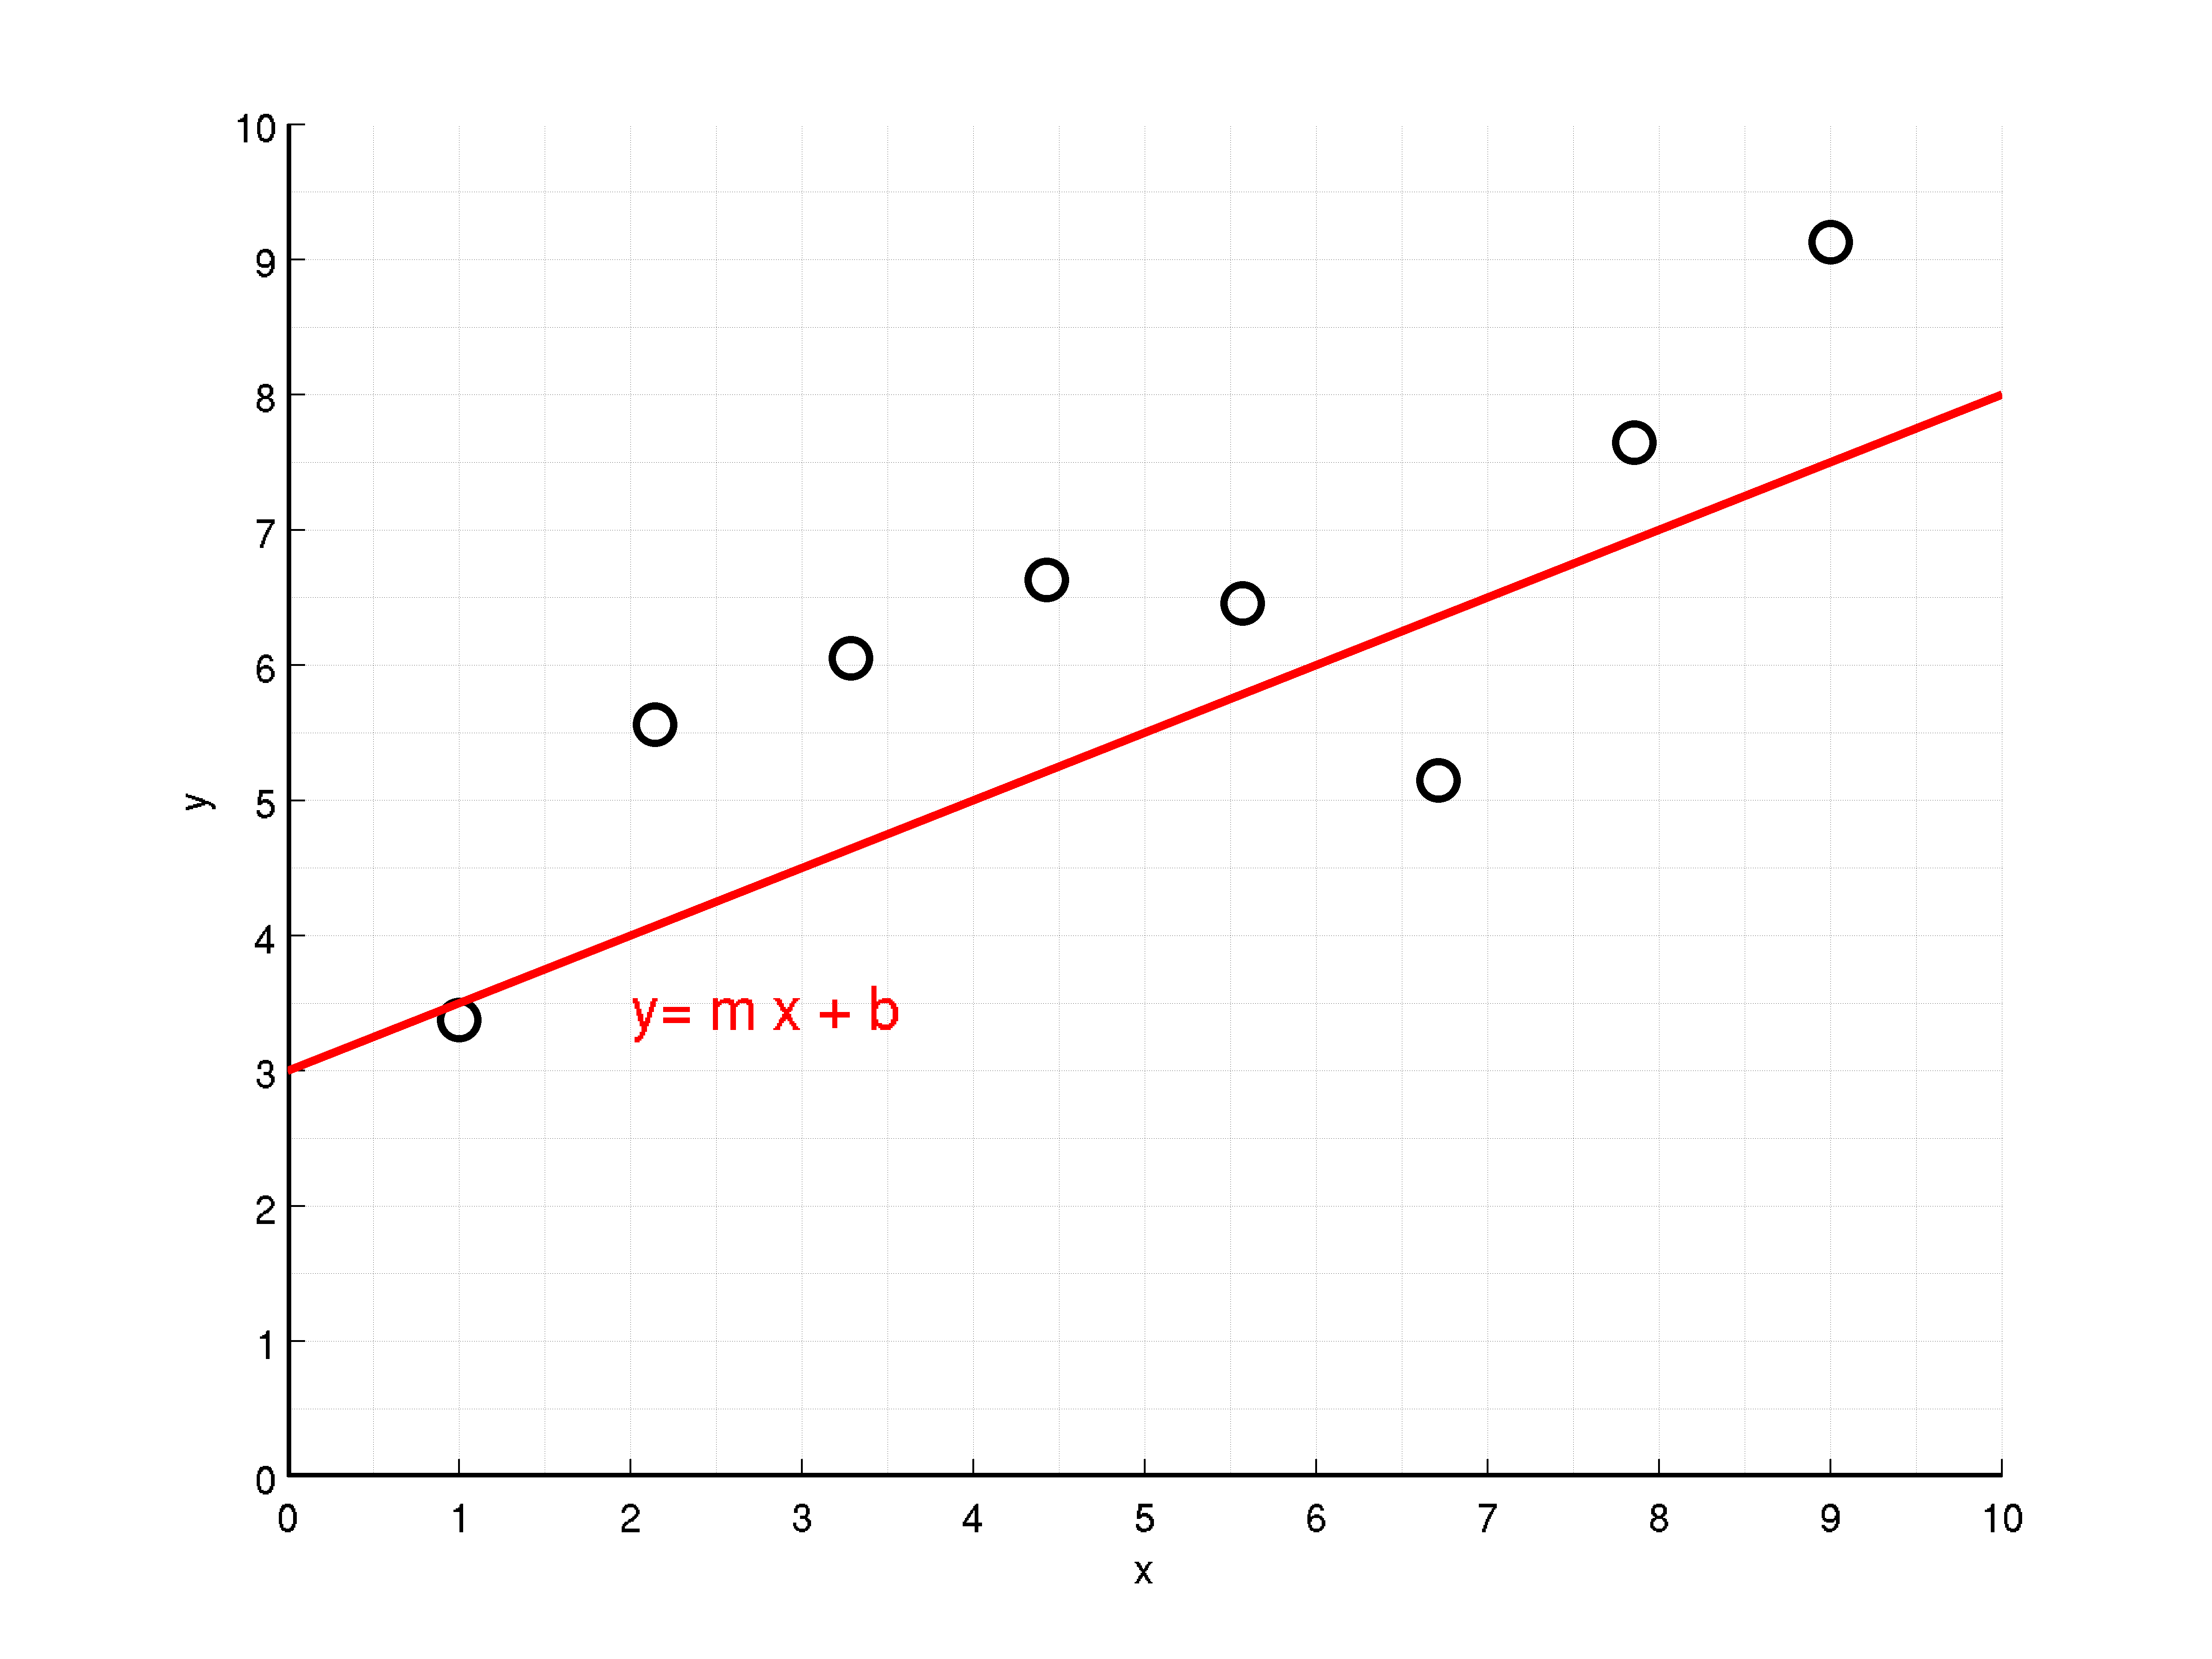
\includegraphics[width=5cm]{img/regressionInferenceOne}}
    }

    \only<3>{%
      \centerline{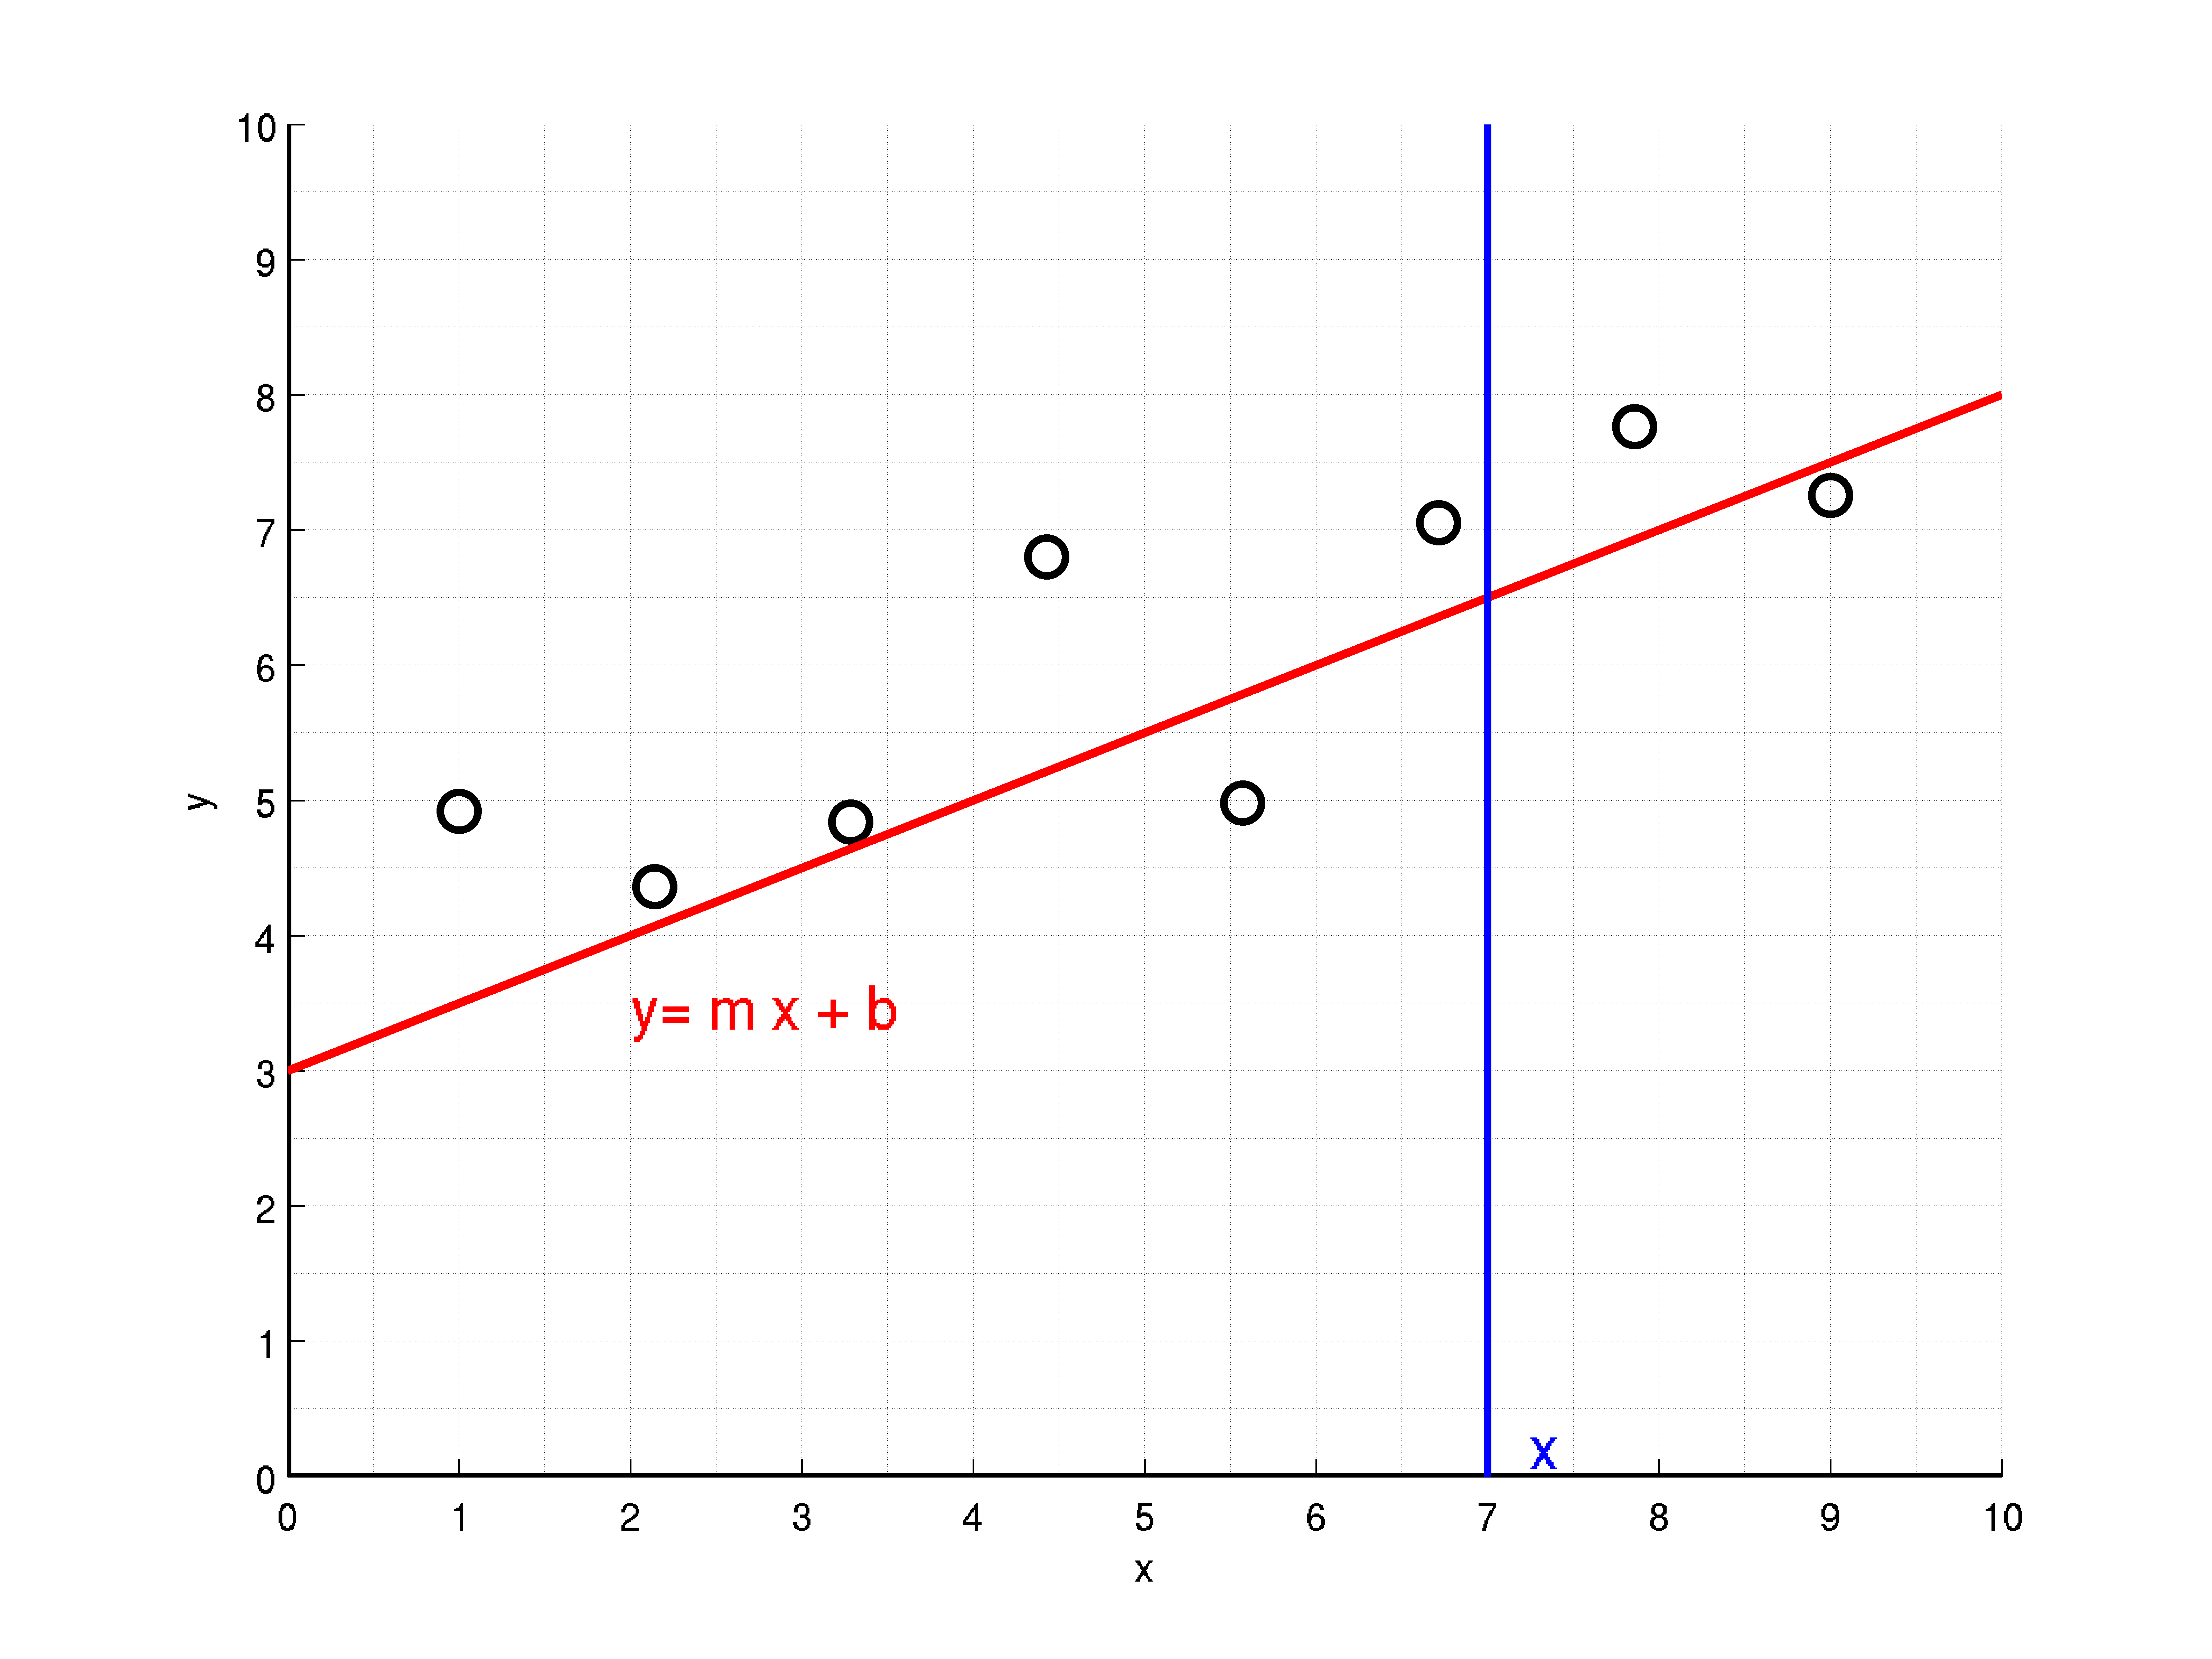
\includegraphics[width=5cm]{img/regressionInferenceTwo}}
    }

    \only<4>{%
      \centerline{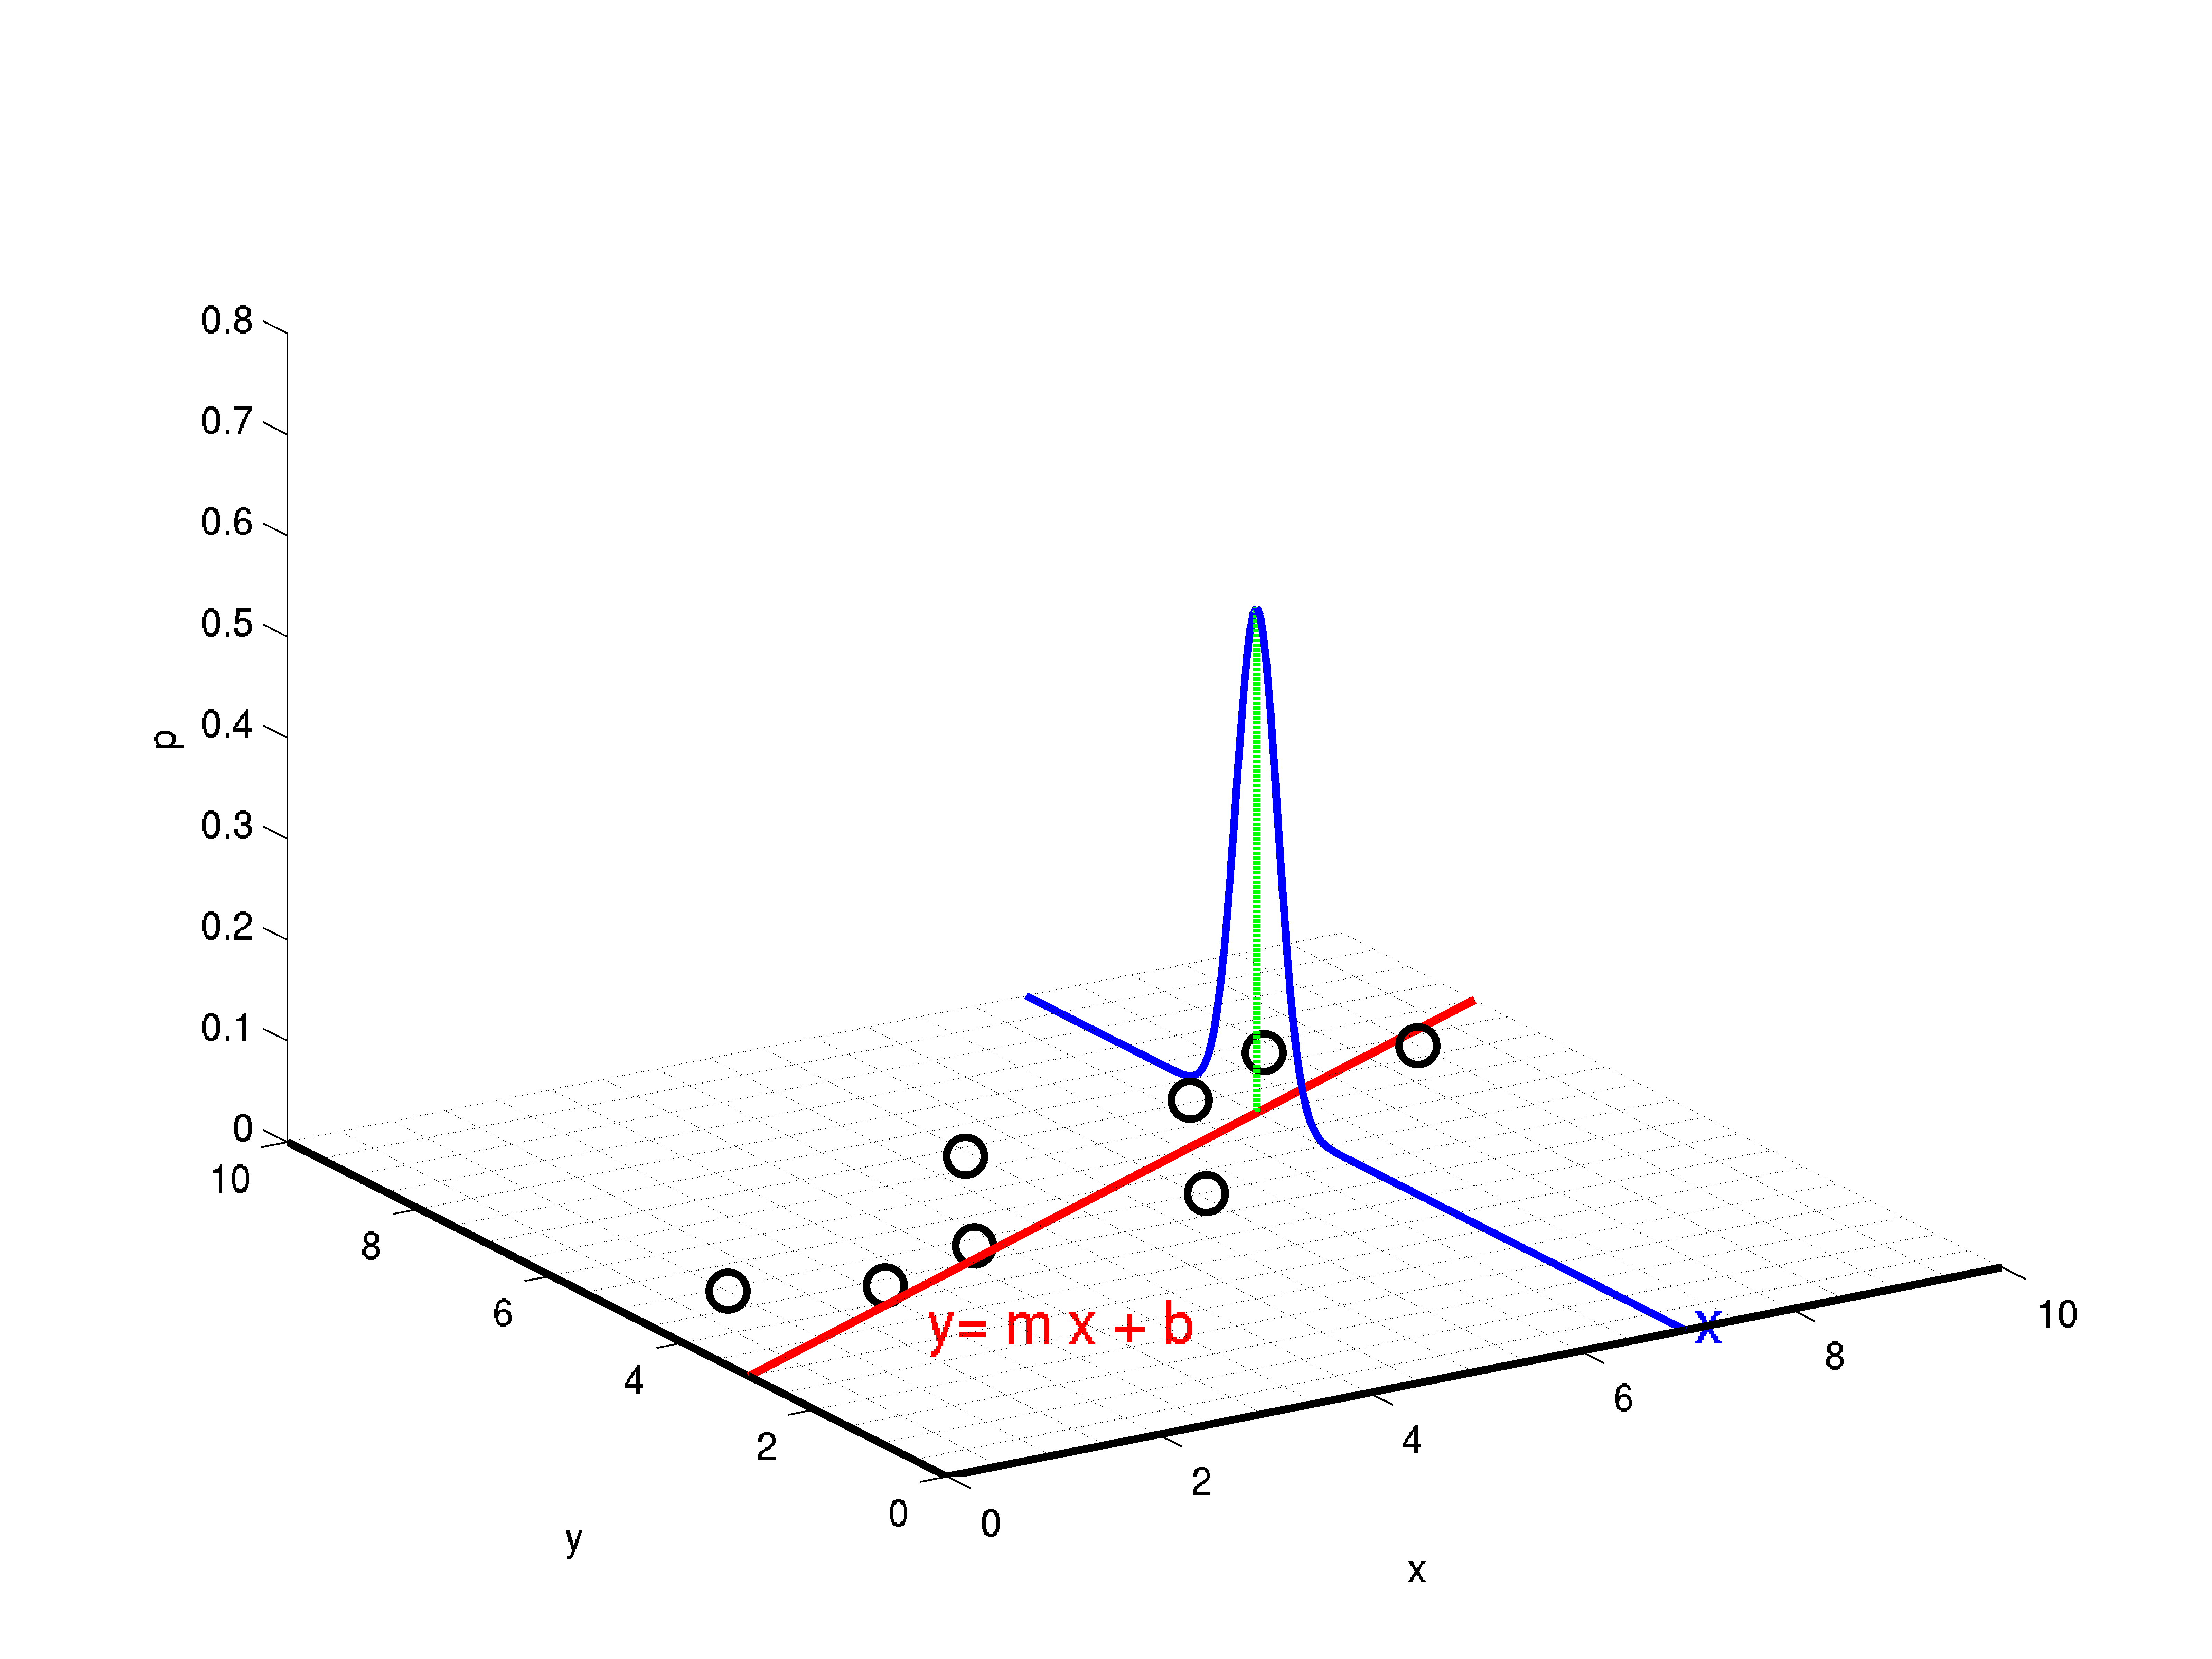
\includegraphics[width=5cm]{img/regressionInferenceThree}}
    }

  
\end{frame}

\begin{frame}
  \frametitle{The Predicted Value}

  The predicted value is 
  \begin{eqnarray*}
    \hat{y} & = & \hat{m} x + \hat{b}.
  \end{eqnarray*}


  The predicted value  satisfies a $t$-distribution by
  \begin{eqnarray*}
    t & = & \frac{\hat{y}-y_{\mathrm{true}}}{s_e \sqrt{\frac{1}{n}+\frac{(x-\bar{x})^2}{S_{xx}}}},
  \end{eqnarray*}
  with $n-2$ degrees of freedom.

\end{frame}


\begin{frame}
  \frametitle{The Predicted Value}

  The predicted value is 
  \begin{eqnarray*}
    \hat{y} & = & \hat{m} x + \hat{b}.
  \end{eqnarray*}



    \begin{columns}

      \column{.5\textwidth}
      Confidence Intervals:
      \begin{eqnarray*}
        t_{cr} & = & \frac{\mathrm{error}}{s_e \sqrt{\frac{1}{n}+\frac{(x-\bar{x})^2}{S_{xx}}}},
      \end{eqnarray*}
      with $n-2$ degrees of freedom.

      \column{.5\textwidth}

      Hypothesis Testing:
      \begin{eqnarray*}
        t & = & \frac{\hat{y}-y_{\mathrm{true}}}{s_e \sqrt{\frac{1}{n}+\frac{(x-\bar{x})^2}{S_{xx}}}},
      \end{eqnarray*}
      with $n-2$ degrees of freedom.

    
    \end{columns}


\end{frame}


\section{Examples}

\begin{frame}{Example}

  \vspace*{-4em}

    \begin{columns}
      \column{.15\textwidth}

      \begin{tabular}{l|l}
        $X$ & $Y$ \\ \hline
        1 &  -4.7 \\
        2 & -15.4  \\
        3 &  -9.6 \\
        4 & -21.5 
      \end{tabular}

      \column{.44\textwidth}

      \begin{eqnarray*}
        \bar{x} & = & 2.5 \\
        \bar{y} & = & -12.8, \\
        s_{xx} & = & 5, \\
        s_{yy} & = & 158.3, \\
        s_{xy} & = & -22.3.
      \end{eqnarray*}

      \column{.44\textwidth}

      \begin{eqnarray*}
        \hat{m} & = & \frac{-22.3}{5}, \\
        \hat{b} & = & -12.8 - \frac{-22.3}{5} \cdot 2.5, \\
        s_e & \approx & 5.42
      \end{eqnarray*}

      \begin{eqnarray*}
      \end{eqnarray*}

    \end{columns}


    \vfill 


    A colleague says that when $x$ is equal to 3.5 then y is -19.2. Is
    he right?

      \only<2>
      {
        \begin{eqnarray*}
          H_0: & & y=-19.2, \\
          H_a: & & y\neq -19.2,
        \end{eqnarray*}
        use $\alpha=0.05$.
      }

      \only<3>
      {
        \begin{eqnarray*}
          t_{cr} & \approx & \pm 4.30 \\
          \hat{y} & = & \frac{-22.3}{5} \cdot 3.5 - 1.65, \\
          t^* & = & \frac{-17.26-(-19.2)}{5.42\sqrt{\frac{1}{4} + \frac{(3.5-2.5)^2}{5}}}, \\
          & \approx &  0.533
        \end{eqnarray*}
      }


      \only<4->
      {
        There is {\color{red}not} sufficient evidence to reject $H_0$
        at the 95\% confidence level assuming a $t$-distribution and 2
        degrees of freedom.
      }


\end{frame}


\begin{frame}{Example}


    \begin{columns}
      \column{.15\textwidth}

      \begin{tabular}{l|l}
        $X$ & $Y$ \\ \hline
        1 & 3 \\
        2 & 5  \\
        3 & 9 \\
        4 & 7  \\
        5 & 10
      \end{tabular}

      \column{.44\textwidth}

      \begin{eqnarray*}
        \bar{x} & = & 3 \\
        \bar{y} & = & 6.8, \\
        s_e & \approx & 1.55 \\
        \hat{m} & = & 1.6, \\
        \hat{b} & = & 2.0.
      \end{eqnarray*}

      \column{.44\textwidth}

      \begin{eqnarray*}
        s_{xx} & = & 10, \\
        s_{yy} & = & 32.8, \\
        s_{xy} & = & 16.
      \end{eqnarray*}

    \end{columns}


    \vfill 


      Find the 95\% confidence interval for the value of $y$ at $x=3.5$.

      \only<2->
      {

        The 95\% confidence interval for the value of $y$ at $x=3.5$
        is between 5.26 and 9.94 assuming a $t$-distribution with 3 d.f..
      }


\end{frame}


\begin{frame}{Example}

  \iftoggle{clicker}{%

    \begin{columns}
      \column{.15\textwidth}

      \begin{tabular}{l|l}
        $X$ & $Y$ \\ \hline
        1 & 3 \\
        2 & 5  \\
        3 & 9 \\
        4 & 7  \\
        5 & 10
      \end{tabular}

      \column{.44\textwidth}

      \begin{eqnarray*}
        \bar{x} & = & 3 \\
        \bar{y} & = & 6.8, \\
        s_e & \approx & 1.55 \\
        \hat{m} & = & 1.6, \\
        \hat{b} & = & 2.0.
      \end{eqnarray*}

      \column{.44\textwidth}

      \begin{eqnarray*}
        s_{xx} & = & 10, \\
        s_{yy} & = & 32.8, \\
        s_{xy} & = & 16.
      \end{eqnarray*}

    \end{columns}


    \vfill 


      Find the 95\% confidence interval for the value of $y$ at
      $x=4.5$.

      \vfill

      \begin{tabular}{l@{\hspace{3em}}l@{\hspace{3em}}l@{\hspace{3em}}l}
        A: .58 to 17.8  & B: 5.99 to 12.41 & C: 8.26 to 12.94
      \end{tabular}


    }

\end{frame}




\subsection{Example}


%%% Local Variables: 
%%% mode: latex
%%% TeX-master: "IntroStats"
%%% End: 

% LocalWords:  pausesection hideothersubsections sectionstyle
